\begin{frame}{$\Upsilon$ yields as function of $p_T$}
  \setlength{\unitlength}{1mm}
  \centering
  \scalebox{0.55 }{
  \begin{picture}(150,120)
    \put(0,0){
      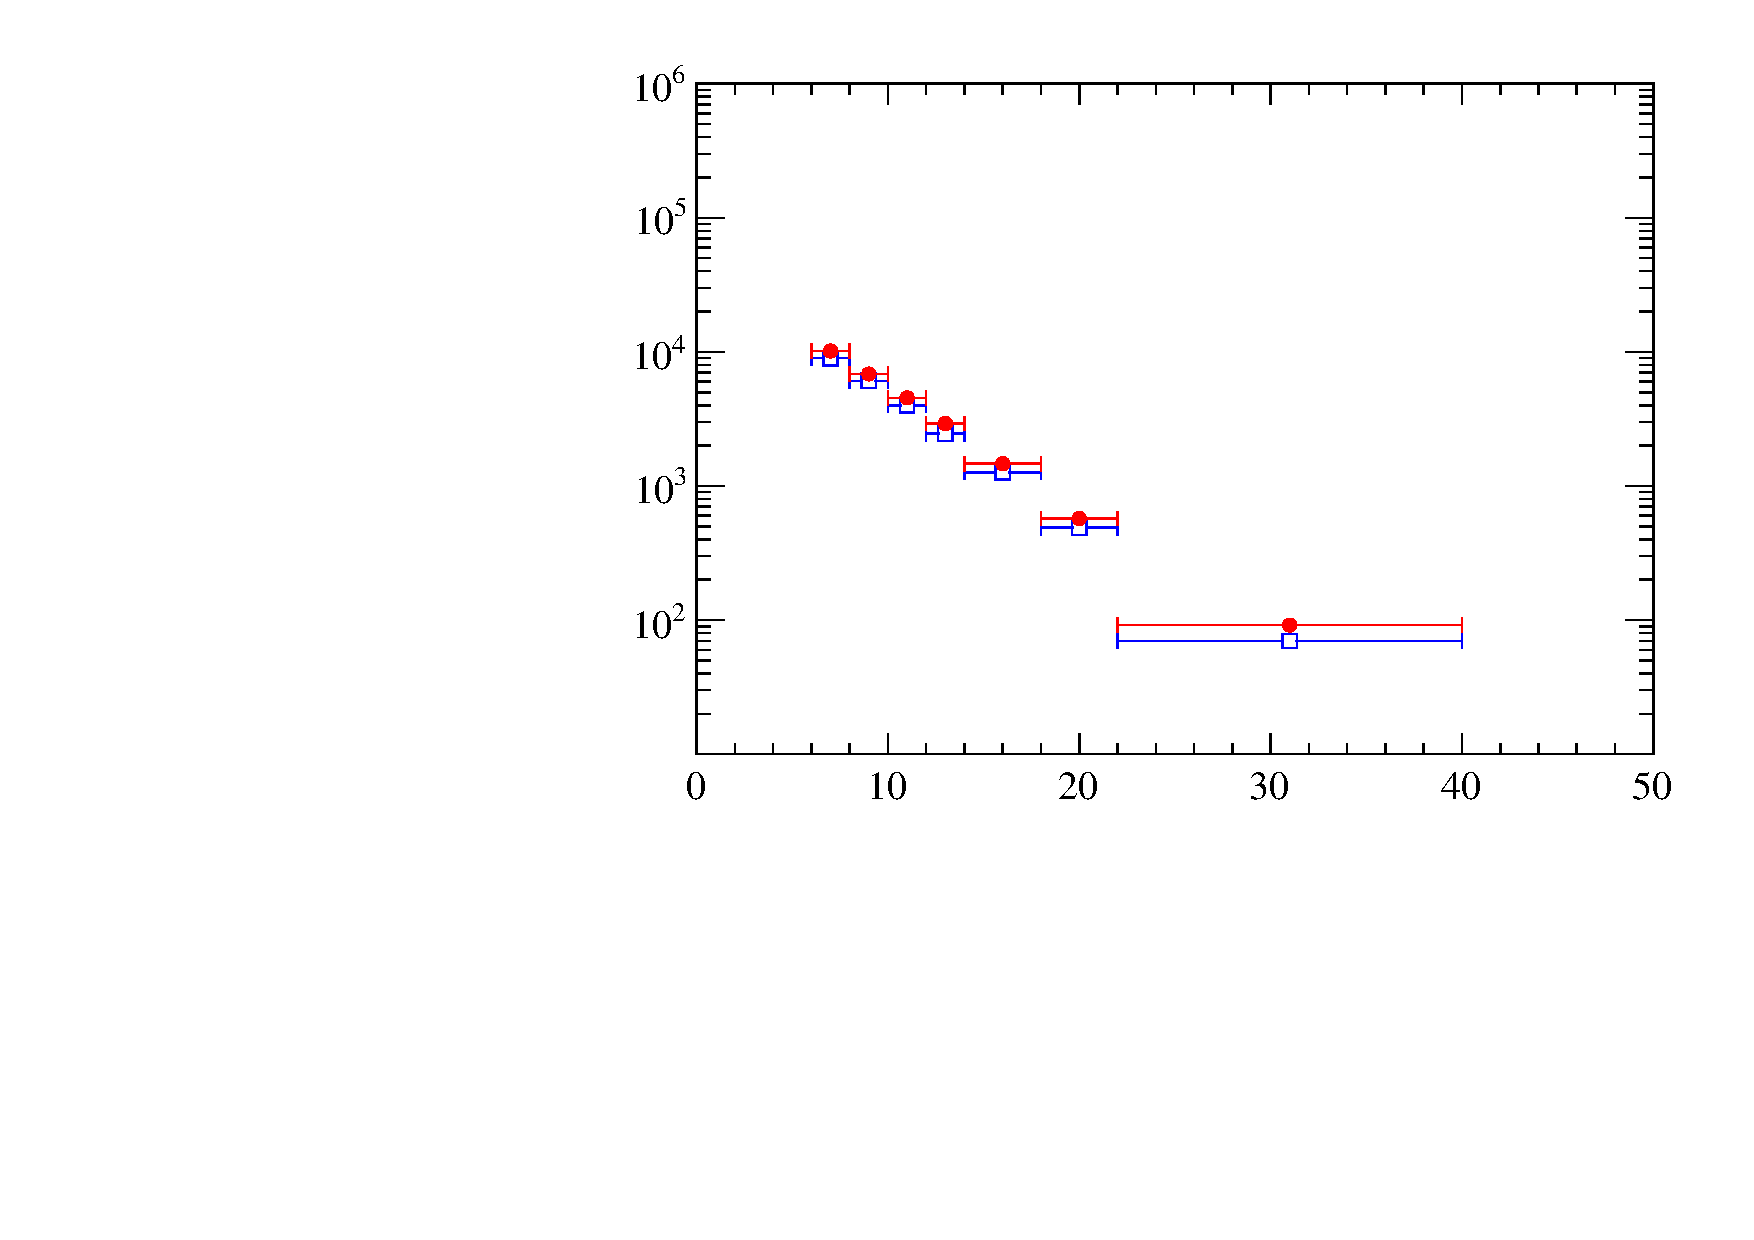
\includegraphics[width=75mm, height=60mm]{upsilon-yields/N3S_scaledbylum}
    }
    \put(0,60){
      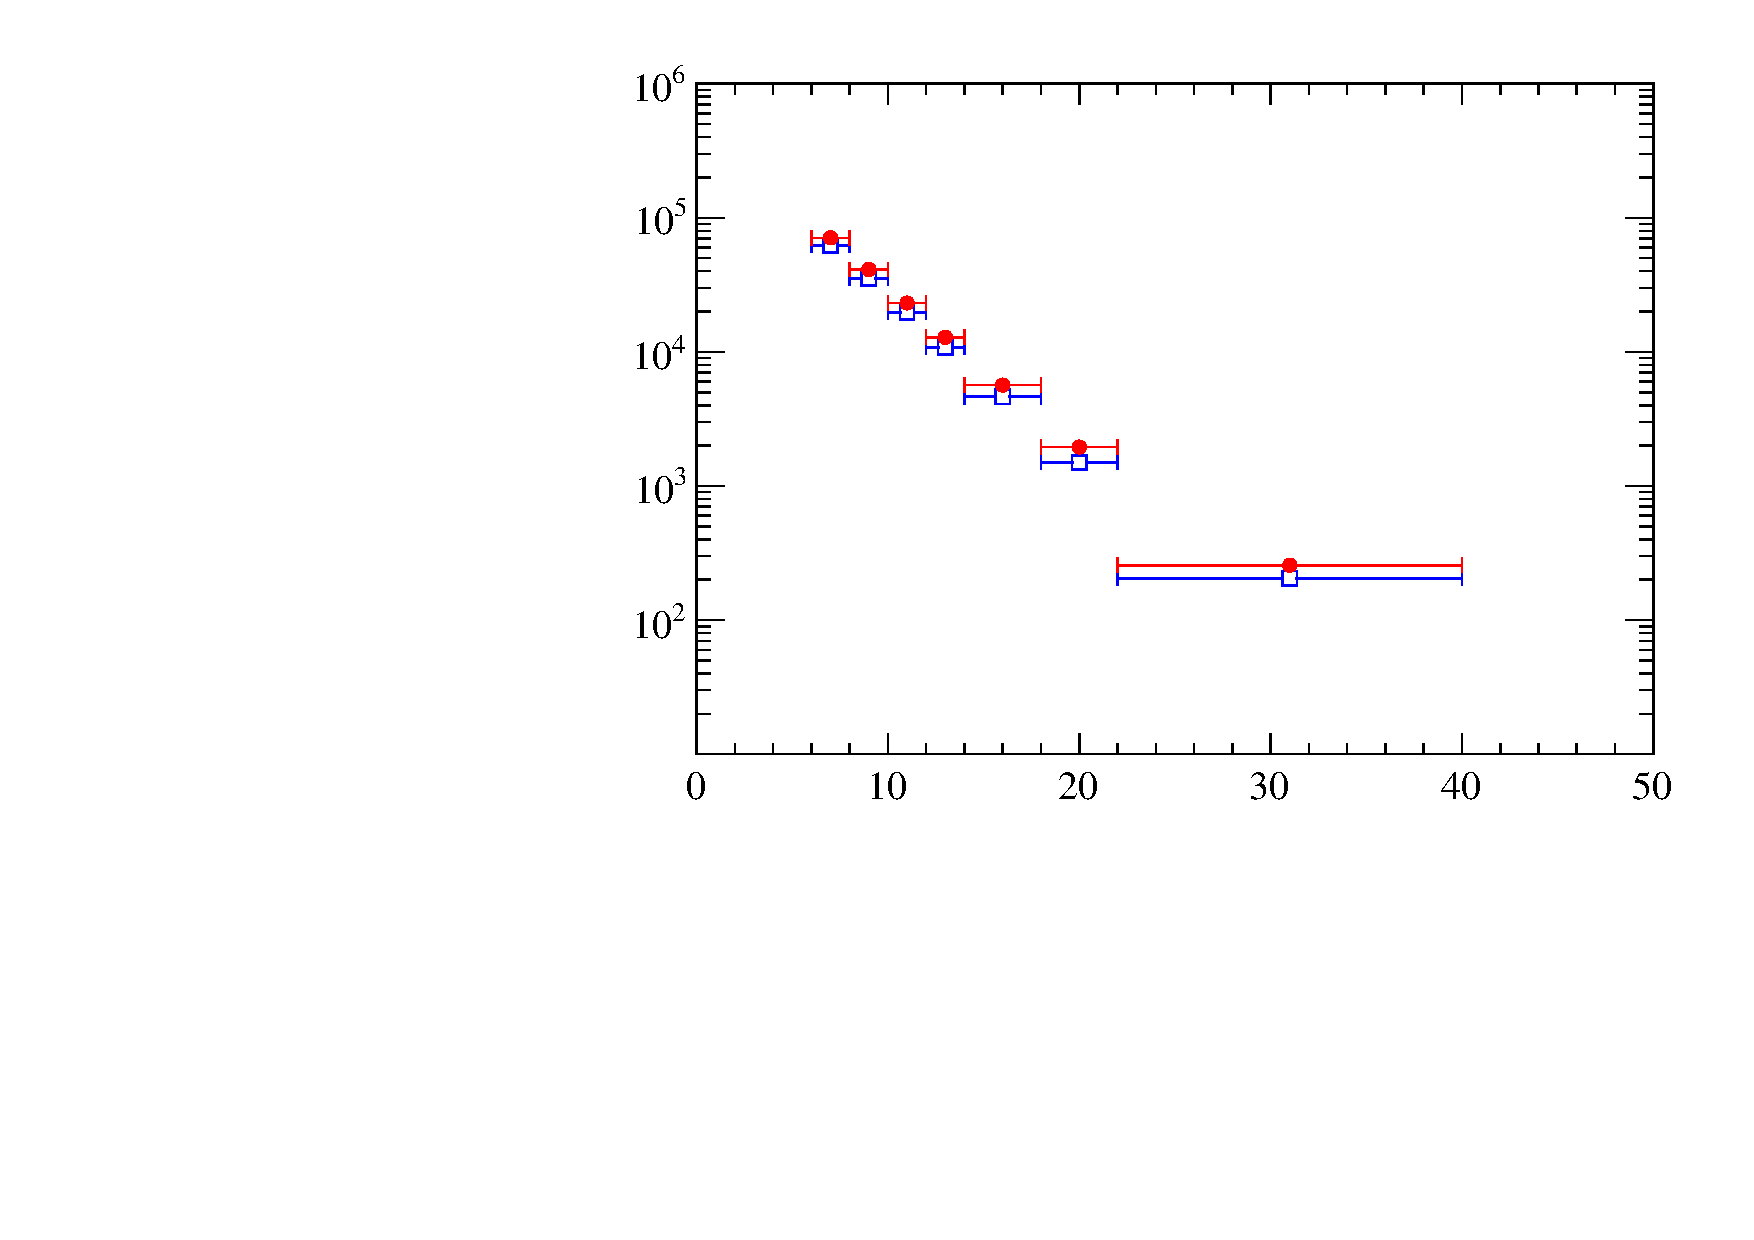
\includegraphics[width=75mm, height=60mm]{upsilon-yields/N1S_scaledbylum}
    }
    \put(75,60){
      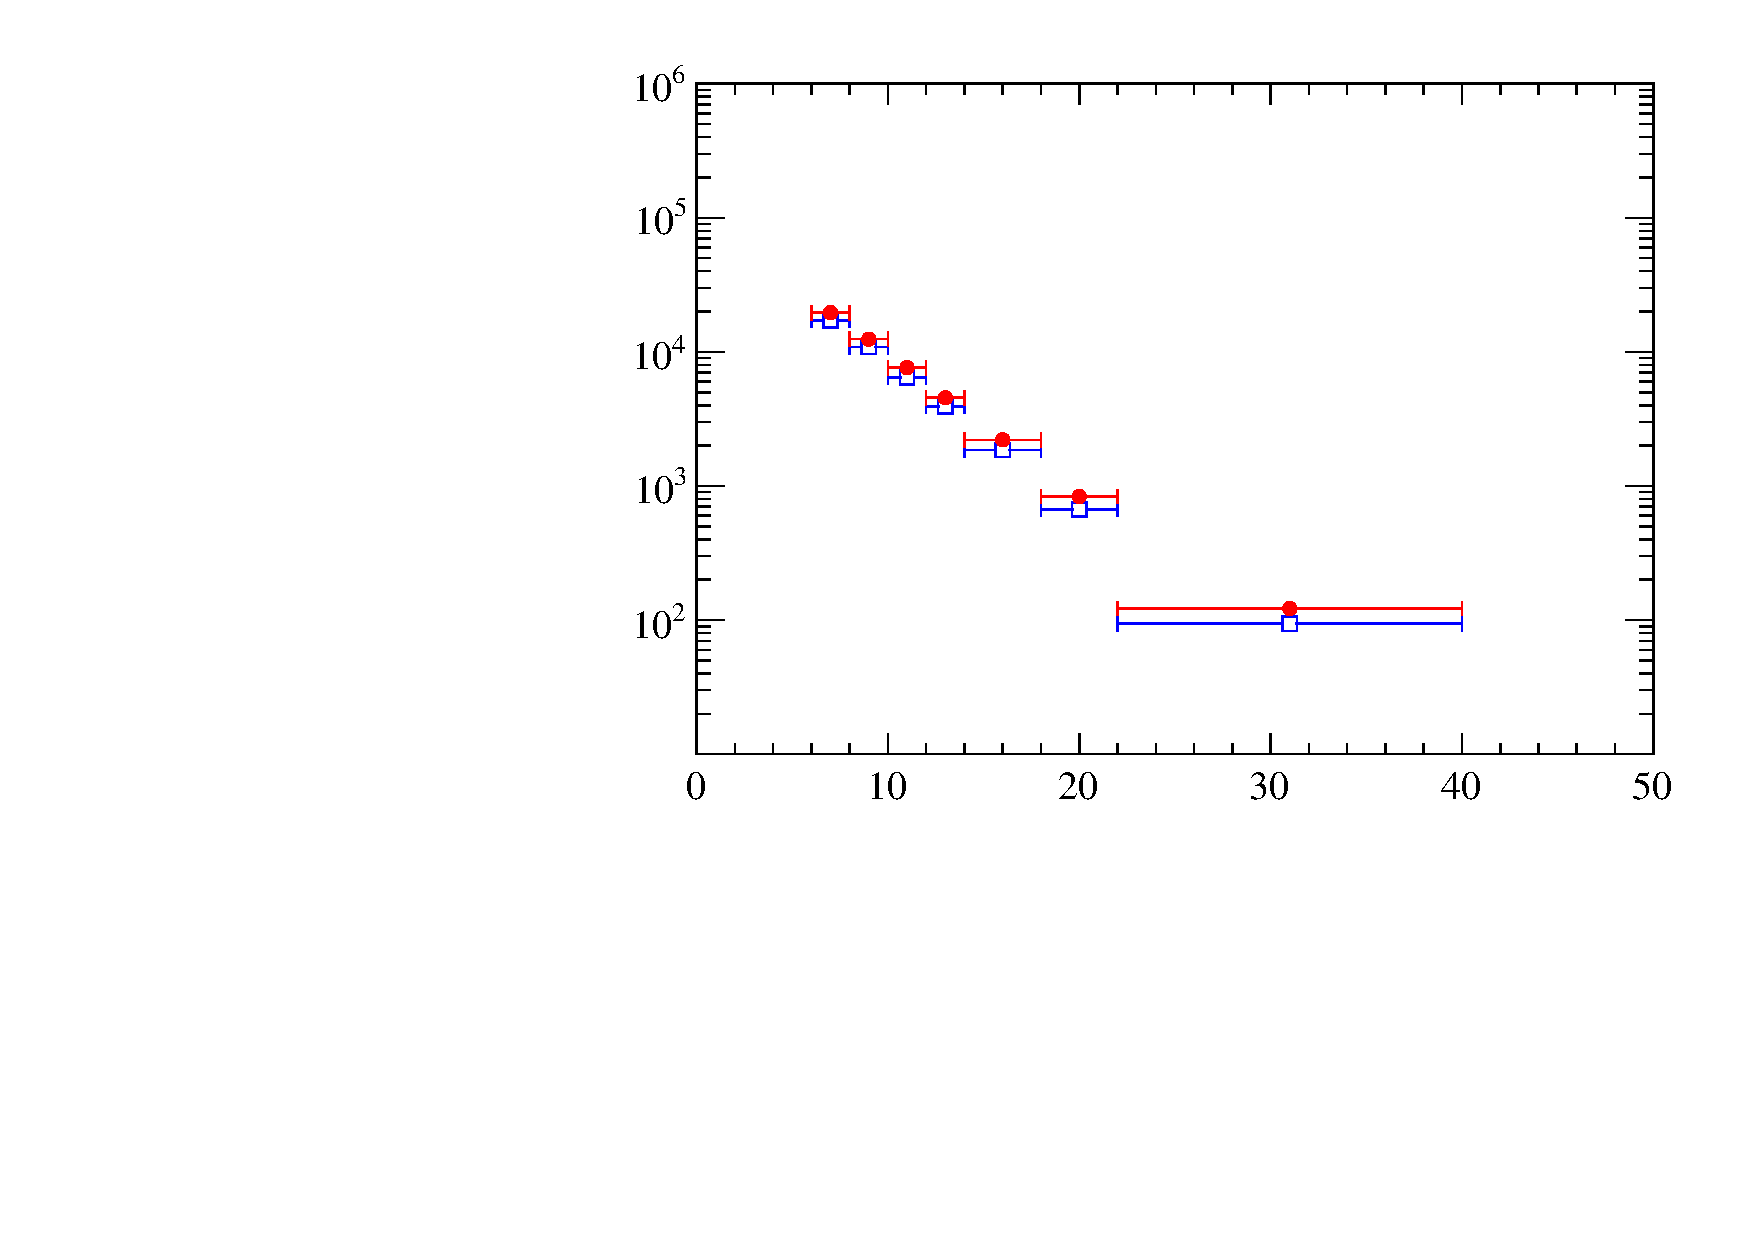
\includegraphics[width=75mm, height=60mm]{upsilon-yields/N2S_scaledbylum}
    }

    \put(2,25){\begin{sideways}Events\end{sideways}}
    \put(35,2){$p_T(\Upsilon) \left[\gevc\right]$}
    \put(55,50){$\Y3S$}

    \put(2,85){\begin{sideways}Events\end{sideways}}
    \put(35,62){$p_T(\Upsilon) \left[\gevc\right]$}
    \put(55,110){$\Y1S$}

    \put(77,85){\begin{sideways}Events\end{sideways}}
    \put(110,62){$p_T(\Upsilon) \left[\gevc\right]$}
    \put(130,110){$\Y2S$}


    \put(50,45){\textcolor{blue}{\sqs=7\tev}}
    \put(50,40){\textcolor{red}{\sqs=8\tev}}
    \put(45,45){
      
\includegraphics[width=3mm, height=2mm]{bsf}
    }
    \put(45,40){
      
\includegraphics[width=3mm, height=2mm]{rco}
    }

    \put(50,105){\textcolor{blue}{\sqs=7\tev}}
    \put(50,100){\textcolor{red}{\sqs=8\tev}}
    \put(45,105){
      
\includegraphics[width=3mm, height=2mm]{bsf}
    }
    \put(45,100){
      
\includegraphics[width=3mm, height=2mm]{rco}
    }

    \put(125,105){\textcolor{blue}{\sqs=7\tev}}
    \put(125,100){\textcolor{red}{\sqs=8\tev}}
    \put(120,105){
      
\includegraphics[width=3mm, height=2mm]{bsf}
    }
    \put(120,100){
      
\includegraphics[width=3mm, height=2mm]{rco}
    }


  % \graphpaper[5](0,0)(75, 60)
  \end{picture}
  }

Yields normalized by bin width and luminosity.

\begin{block}{}
The small difference between 7 and 8\tev data is due to the production cross
sections, which are expect to be about 10\% larger.
\end{block}
 
\end{frame}

